\documentclass[tikz,border=3mm,multi=tikzpicture]{standalone}
\usepackage[utf8]{inputenc}
\usepackage[T1]{fontenc}
\usepackage{helvet}
\renewcommand{\familydefault}{\sfdefault}
\usepackage{tikz}
\usetikzlibrary{arrows.meta,positioning}
\begin{document}

\tikzset{every node/.append style={font=\sffamily\small}}

% TikZ 1
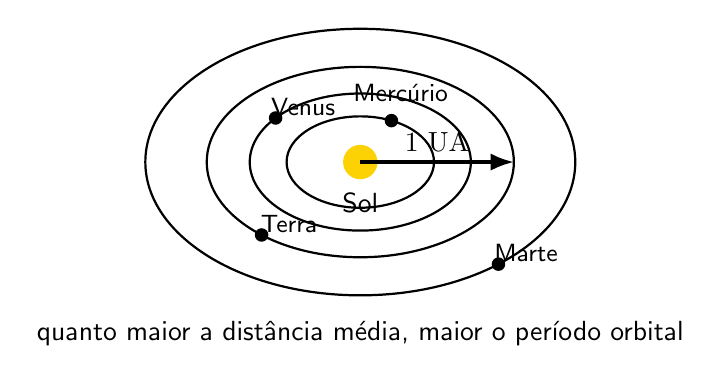
\begin{tikzpicture}[scale=0.78,>=Latex]
  \fill[yellow!70!orange] (0,0) circle (0.28);
  \node[below] at (0,-0.35) {Sol};
  \foreach \r/\name/\ang/\color/\dx/\dy in {1.2/Mercúrio/65/gray/0.15/0.45,1.8/Venus/140/orange/0.45/0.18,2.5/Terra/230/blue/0.45/0.18,3.5/Marte/310/red/0.45/0.18}{
    \draw[thick,\color] (0,0) ellipse ({\r} and {0.62*\r});
    \fill[\color] ({\r*cos(\ang)},{0.62*\r*sin(\ang)}) circle (0.11);
    \node[font=\small] at ({\r*cos(\ang)+\dx},{0.62*\r*sin(\ang)+\dy}) {\name};
  }
  \draw[->,very thick] (0,0) -- (2.5,0) node[midway,above] {$1\ \mathrm{UA}$};
  \node[align=center] at (0,-2.8) {quanto maior a distância média, maior o período orbital};
\end{tikzpicture}

% TikZ 2
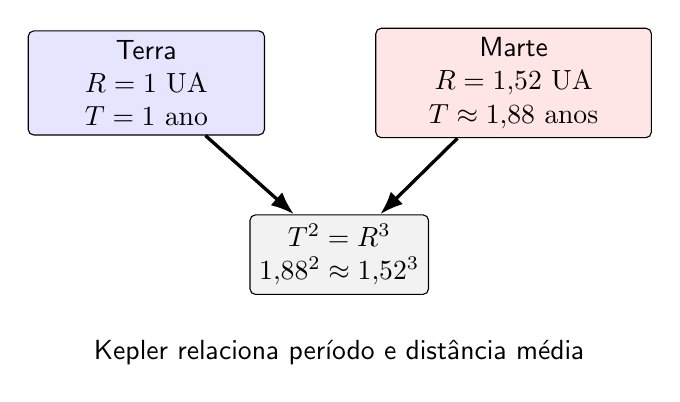
\begin{tikzpicture}[>=Latex,node distance=1cm]
  \node[draw,rounded corners=2pt,fill=blue!10,minimum width=3cm,minimum height=1.1cm,align=center] (terra)
    {Terra\\$R=1\ \mathrm{UA}$\\$T=1\ \mathrm{ano}$};
  \node[draw,rounded corners=2pt,fill=red!10,minimum width=3.5cm,minimum height=1.1cm,align=center,right=1.4cm of terra] (marte)
    {Marte\\$R=1{,}52\ \mathrm{UA}$\\$T\approx1{,}88\ \mathrm{anos}$};
  \node[draw,rounded corners=2pt,fill=gray!10,align=center,below=1cm of terra,xshift=2.45cm] (lei)
    {$T^2 = R^3$\\$1{,}88^2 \approx 1{,}52^3$};
  \draw[very thick,->] (terra) -- (lei);
  \draw[very thick,->] (marte) -- (lei);
  \node[align=center,below=0.45cm of lei] {Kepler relaciona período e distância média};
\end{tikzpicture}

\end{document}
